\chapter{Preliminary}\label{preliminary}
In order to understand the topic of variational autoencoders or even autoencoders in general, we need to consider a couple of preliminary ideas. Those ideas consist mainly of neural networks and their optimization - usually being called training. In this chapter, we will tackle the conceptional idea of how to formulate neural networks in a mathematical way and further, we will consider a couple of useful operations that neural networks are capable of doing. Lastly, we will take a look at some strategies of training neural networks.

\section{Neural networks}
Originally, the idea of neural networks came from analysing mammal's brains. An accumulation of nodes - so called neurons, connected in a very special way that fire an electric impulse to adjacent neurons upon being triggered and transmit information that way. Scientist tried to mimic this natural architecture and replicate the human intelligence artificially. This research has been going for almost 80 years and became immensely popular recently through artificial intelligences like OpenAI's ChatGPT or Google's Bard. But what do these neural networks do? Why are they so popular? What actually is a neural network? All those are very interesting and important questions that we will find answers for.\\
As already mentioned, neural networks consist of single neurons that move around information upon being \glqq triggered\grqq{}. Obviously, triggering an artificial neuron can't happen the same way as neurological neurons are being triggered. Hence, we need to model the triggering of a neuron in some way. The idea is to filter information that does not exceed a certain stimulus threshold. This filter is usually being called activation function. Indeed, there are lots of ways of modelling such activation functions and it primarily depends on the specific use-case what exactly the activation function has to fulfil. Therefore, we define activation functions in the most general way possible.\\
\textcolor{red}{TODO:} Give a formal reference to neural networks somewhere?

\begin{definition}
A non-constant function $\f: \R \to \R$ is called an \textbf{activation function} if it is continuous.
\end{definition}


Even though there is a zoo of different activation functions, we want to consider mainly the following ones.


\begin{example}
The following functions are activation functions.
\begin{mydescription}{\widthof{\textbf{Leaky rectified linear unit (Leaky ReLU)}}}
\item[\textbf{Rectified linear unit (ReLU)}] $\f(t) = \max\{0, t\}$,
\item[\textbf{Leaky rectified linear unit (Leaky ReLU)}] $\displaystyle \f(t) = \begin{cases}
\a t, 	& t \leq 0,\\
t,		& t > 0.
\end{cases}$
\end{mydescription}
\end{example}


Now, having introduced activation functions we can introduce neurons.


\begin{definition}
Let $\f: \R \to \R$ be an activation function and $w\in \R^k$, $b \in \R$. Then a function $h: \R^k \to \R$ is called \textbf{$\f$-neuron} with weight $w$ and bias $b$, if
\begin{align}\label{def_neuron}
h(x) = \f \left(\langle w, x \rangle + b \right), \qquad x \in \R^k.
\end{align}
We call $\t \coloneqq (w, b)$ the parameters of the neuron $h$.
\end{definition}


In order to expand the architecture, we consider multiple neurons being arranged in a so called layer.


\begin{definition}\label{def_layer}
Let $\f: \R \to \R$ be an activation function and $W \in \R^{m\times k}$, $b\in \R^m$. Then a function $H:\R^k \to \R^m$ is called \textbf{$\f$-layer} of width $m$ with weights $W$ and biases $b$ if for all $i=1,\ldots,m$ the component function $h_i$ of $H$ is a $\f$-neuron with weight $w_i = W^\top e_i$ and bias $b_i = \langle b, e_i \rangle$, where $e_i$ denotes the standard ONB of $\R^m$.\\
If we consider $\hat{\f}: \R^k \to \R$ as the component-wise mapping of $\f:\R\to \R$, meaning $\hat{\f}(v) = (\f(v_1), \ldots, \f(v_k))$, we can generalize the $\f$-layer $H:\R^k \to \R^m$ by
\begin{align}
H(x) = \hat{\f}(Wx + b), \qquad x \in \R ^k.
\end{align}
\end{definition}


Finally, we can introduce neural networks with the previous definitions formally.


\begin{definition}
Let $\f: \R \to \R$ be an activation function and $H_1, \ldots, H_L$ with $L \in \N$ be $\f$-layers with parameters $\t_i = (W_i, b_i)$ as in definition \ref{def_layer}. Then, with $\t = (\t_1, \ldots \t_L)$ the function $f_{\f, L, \t}: \R^{d_1} \to \R^{d_L}$ defined by
\begin{align}
f_{\f, L, \t} (x) \coloneqq H_L \circ \ldots \circ H_1 (x), \qquad x \in \R^{d_1},
\end{align}
is called a \textbf{$\f$-deep neural network} of depth $L$ with parameters $\t \in \T$, where $d_1$ describes the input dimension and $d_L$ the output dimension respectively and $\T$ is some arbitrary parameter space.\\
Lastly, we will write $f\coloneqq f_{\f, L, \t}$, if the activation function $\f$, the depth $L$ and the parameters $\t$ are clear out of context.
\end{definition}


A visual representation of a neural network can be found in figure \ref{img_nn}


\begin{figure}[H]
\begin{center}
   \begin{minipage}[b]{0.9\linewidth}
      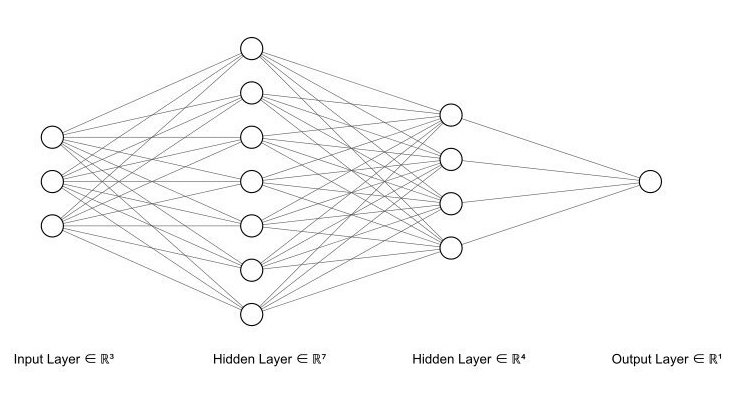
\includegraphics[width=\linewidth]{neural_net}
      \caption{A neural network with input $x\in \R^4$ and output $y\in\R^2$. The five hidden layers have dimensions $3$, $4$, $5$, $3$ and $7$ respectively. The graphic was generated with http://alexlenail.me/NN-SVG/index.html}\label{img_nn}
	\end{minipage}
\end{center}
\end{figure}


\section{Training of neural networks}

Since we now know what neural networks are, we want to discuss how to tune them to a specific problem. This procedure is usually called training of a neural network. There are many approaches of how to train a neural network. However, most of them rely on iteratively finding the gradient - the direction of greatest ascent. In the following we want to consider a couple of popular algorithms that are used to train neural networks.


\begin{theorem}\label{theorem_gd}
Let $(\g_t)_{t \in \N}$ be a converging sequence of step sizes with $\g_t \to 0$. Let further be $f:\R^n \to \R$ a continuous, convex and differentiable function. Furthermore, let $x^{(t)}$ denote the $t$-th iterate of the \textbf{gradient descent algorithm} defined by
\begin{align}
x^{(t+1)} = x^{(t)} - \g_t \partial_x f(x^{(t)}),
\end{align}
with a suitable initial guess $x^{(0)}\in \R^n$.\\
Then the algorithm converges to the global minimum $f(x^{\ast})\in \R$, meaning
\begin{align*}
x^{\ast} \coloneqq \argmin_{x\in\R^n}f(x) = \lim_{t\to\infty} x^{(t)}.
\end{align*}
Lastly, if the function $f$ is strictly convex, then the global minimum $f(x^{\ast)}\in\R$ is unique.
\end{theorem}


\begin{proof}
If the step size is sufficiently small such that the iterate is contained in the sphere around $x^{\ast}$ with radius $d\left(x^{\ast}, x^{(t)}\right)$,
the iterate $x^{(t+1)}$ is bound by a sphere around $x^{\ast}$ with radius $d\left(x^{\ast}, x^{(t)} - \g_t \nabla_x f(x^{(t)})\right) < d\left(x^{\ast}, x^{(t)}\right)$, since
\begin{align*}
d\left(x^{\ast}, x^{(t)}\right) &\geq d\left(x^{\ast}, x^{(t+1)}\right)\\
&= d\left(x^{\ast}, x^{(t)} - \g_t \nabla_x f(x^{(t)})\right).
\end{align*}
Hence, the distance $d(x^{\ast}, x^{(t)})$ becomes smaller in each iteration, due to the convexity of $f$, with
\begin{align*}
\lim_{t\to\infty} d\left(x^{\ast}, x^{(t)}\right) = 0,
\end{align*}
since we know that $\R^n$ is a Banach space and $\left(d\left(x^{\ast}, x^{(t)}\right)\right)_{t\in\N}$ is a converging sequence by construction.\\
It is left to show, that if the function $f$ is strictly convex, then the global minimum $f(x^{\ast})\in\R$ is unique. This assertion holds, since if there were two global minima $f\left(x_1^{\ast}\right), f\left(x_2^{\ast}\right)$ with $x_1^{\ast} \neq x_2^{\ast}$.\\
Now consider $x^{\prime} \coloneqq \frac{x_1^{\ast} + x_2^{\ast}}{2}$, a point between $x_1^{\ast}$ and $x_1^{\ast}$. Since $f$ is assumed to be strictly convex, this leads to
\begin{align*}
f\left(x^{\prime} \right) = f\left(\frac{1}{2}x_1^{\ast} + \frac{1}{2} x_2^{\ast}\right) < \frac{1}{2} f\left(x_1^{\ast} \right) + \frac{1}{2} f\left(x_2^{\ast}\right) = f\left(x_1^{\ast}\right) = f\left(x_2^{\ast}\right).
\end{align*}
This would contradict the assumption that $f\left(x_1^{\ast}\right), f\left(x_2^{\ast}\right)$ are minima, especially global minima. Hence, the assertion holds.
\end{proof}


Since we are considering neural networks in this thesis, we want to take a quick look on how we can apply theorem \ref{theorem_gd} to a neural network. But firstly, we need to define the so called loss function and risk function - functions to measure the error of a neural network, or any prediction function in general. This is fundamental in supervised learning.


\begin{definition}\label{def_loss_risk}
Let $X\subseteq \R^d$ and $Y \subseteq \R^n$ be arbitrary Banach spaces and $d, n \in \N$, that we will refer to as input and output space, $p:X \to \R^n$ be a continuous, convex function.\\
Furthermore, let $L: X \times Y \times \R^n \to [0, \infty)$ be a \textbf{loss function}, a measurable function that compares a true value $y \in Y \subset \R^n$ to a predicted value $\hat{y} = p(x)$.\\
Lastly, let $\prob$ be a probability measure on $X \times Y$. Then the \textbf{$L$-risk function} $\risk: X \times Y \times \R^n \to [0, \infty)$ with regard to a loss function $L$ is defined as
\begin{align*}
\risk_{L, \prob}(p) = \int_{X\times Y} L\left(x, y, p(x) \right) d \prob(x, y).
\end{align*}
\end{definition}


In applications one usually wants to compute the risk with regard to some observed data. In this case the general definition of a risk function becomes more tangible, as we see in the following definition.


\begin{definition}\label{def_empirical_risk}
Let $X\subseteq \R^d$ and $Y \subseteq \R^n$ be arbitrary Banach spaces and $d, n \in \N$, $D = \left((x_1,y_1), \ldots, (x_k,y_k)\right)$ be a dataset consisting of $k\in\N$ data points. Furthermore, let $L$ be a loss function and $p$ be an arbitrary prediction function as in definition \ref{def_loss_risk}.\\
Then we define the \textbf{empirical risk function} as
\begin{align}
\risk_{L, D} (p) = \frac{1}{k} \sum_{i=1}^{k} L\left(x_i, y_i, p(x_i)\right).
\end{align}
Since we will mostly consider the practical setting where we have a dataset given, we will write $\risk \coloneqq \risk_{L, D}$ unless unclear in the given context.
\end{definition}


With the above definitions we now need to consider one last thing in order to formulate the gradient descent algorithm for neural networks. This last thing is the question how actually to compute the gradient of a neural network.


\begin{lemma}\label{nn_gradient}
Let $f_\t:\R^d\to \R$ be a neural network with parameters $\t\in\T$, arbitrary depth $L\in\N$ and arbitrary activation function $\f$. Furthermore, let $D$ be a dataset of length $k\in \N$ and $L$ be an arbitrary loss function as in definition \ref{def_loss_risk}.\\
The gradient of the risk function $\risk(\cdot)$ with regard to the neural network $f_\t$ and thus the parameters $\t$ looks as follows
\begin{align*}
\partial_\t \risk \left(f_{\t}\right) = \frac{1}{k} \sum_{i=1}^{k} \partial_\t L\left(x_i, y_i, f_\t(x_i)\right).
\end{align*}
Hence, it is the average of gradients in all data points $(x_i,y_i) \in D$.
\end{lemma}


\begin{proof}
To prove the assertion we simply use the definition \ref{def_empirical_risk} of the empirical risk function and consider the linearity property of derivatives.
\begin{align*}
\partial_\t \risk \left(f_{\t}\right) &= \partial_\t \frac{1}{k} \sum_{i=1}^{k} L\left(x_i, y_i, f_\t(x_i)\right)\\
&= \frac{1}{k} \sum_{i=1}^{k} \partial_\t L\left(x_i, y_i, f_\t(x_i)\right)
\end{align*}
\end{proof}


With the above definitions we now can formulate the gradient descent algorithm for a neural network.


\begin{corollary}
Let $f_\t:\R^d\to \R$ be a neural network with parameters $\t\in\T$, arbitrary depth $L\in\N$ and arbitrary activation function $\f$. Let $(\g_t)_{t \in \N}$ be a converging sequence of step sizes with $\g_t \to 0$ and $D$ be a dataset of length $k\in \N$.\\
Then one can train the neural network $f_\t$ with the gradient descent algorithm proposed in theorem \ref{theorem_gd}. In this setting, the algorithm looks as follows
\begin{align*}
\t^{(t)} = \t^{(t - 1)} - \g_{t-1} \partial_\t \risk \left(f_{\t^{(t -1)}}\right),
\end{align*}
where the gradient can be computed as in lemma \ref{nn_gradient}
\end{corollary}


\textcolor{red}{TODO:} Name some properties (convergence, rate, etc.) and reference them


This is a valuable result, since this way one can iteratively optimize any convex function. Such iterative methods are powerful in numerical settings, where one could use a machine to compute the result. However, there is one problem: in many practical cases it is way to costly to compute the gradient, if the dataset becomes significantly large. This lead to a bunch of approaches on how to make this algorithm more efficient, one of those being the following.

\begin{theorem}
Let $f_\t:\R^d\to \R$ be a neural network with parameters $\t\in\T$, arbitrary depth $L\in\N$ and arbitrary activation function $\f$. Let $(\g_t)_{t \in \N}$ be as previous and $D$ be a dataset of length $k\in \N$.\\
Then we define the $t$-th iterate of the \textbf{stochastic gradient descent algorithm} by
\begin{align}
\t^{(t)} = \t^{(t - 1)} - \g_{t-1} \partial_{\t, i} \risk \left(f_{\t^{(t - 1)}}\right),
\end{align}
with $i \in \{1,\ldots, k\}$ and $\partial_{\t, i} \risk \left(f_{\t^{(t)}}\right)$ denoting the gradient with regard to the $i$-th data tuple $(x_i, y_i) \in D$.
\end{theorem}


\textcolor{red}{TODO:} Name some properties (convergence, rate, etc.) and reference them \\
\textcolor{red}{TODO:} Since ADAM optimizers perform best at the current state of the art, it would be nice to see how it works. However, it would need come pages to introduce.. Is it worth it?

\section{Neural networks in computer vision}

Lastly in this chapter, we want to apply the theory of neural networks to the setting we actually are interested in. This setting is usually called computer vision - basically, Machine Learning that is applied to images and videos. Since we want to apply neural networks to a problem that has to do with images, we need to know how to see an image in a mathematical way.

\begin{definition}
Let $M,N\in\N$ and $\O=\{1,\ldots,M\}\times \{1,\ldots,N\} \subset \N^2$ be called \textbf{pixel domain} of an image with the tuple $(M,N)$ being called \textbf{resolution}. Then we define a \textbf{digital image} by $(\p)_{i,j} \in \P_d \coloneqq \{1,\ldots,255\}^d$ for all $(i,j)$ in $\O$, where $d\in\N$ represents the number of \textbf{channels} in each pixel.\\
We will denote $\p\in\P_{d,\O}\coloneqq \P_d^{M\times N}$ from now on.
\end{definition}

\begin{remark}
We want to distinguish two kinds of pictures. If $d=1$, we speak of a \textbf{black and white picture}.\\
If $d=3$, we speak of an \textbf{RGB picture}. Here, RGB stands for the  red, green and blue color channels.
\end{remark}

Now having formally defined what an image is, we can consider how a neural network operating on images looks like. In order to do this, it is sufficient to consider how a neural layer operating on images looks like.

\begin{corollary}
Let $\f$ be an arbitrary activation function and $\O_0$ be an arbitrary pixel domain with resolution $(M_0,N_0)\in\N^2$. Let $\p$ be an image with number of channels $d\in\N$.\\
Since we will not change the number of channels throughout the neural network, we reduce $\P_{d_\O}$ to $\P_{\O}$. Then a neural layer that operates on images looks as follows
\begin{align*}
H: \P_{\O_0} &\to \P_{\O_1}\\
\p_0 &\mapsto \p_1,
\end{align*}
where $\p_1$ is an image on the pixel domain $\O_1$ with resolution $(M_1,N_1)\in\N^2$

\end{corollary}
